\section{Data Preprocessing}

\begin{remark}
    Learning Objectives:
    \begin{itemize}
        \item Understand fundamental importance of data preprocessing
        \item Know basic algorithms for data cleaning, (near) duplicate detection and filling missing values
    \end{itemize}
\end{remark}

\subsection{Data}

\begin{concept}{Typical Data Driven Project}

    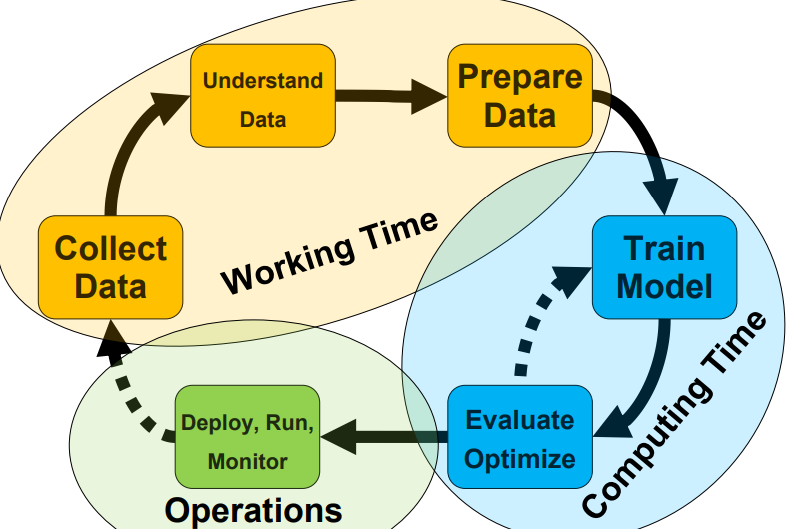
\includegraphics[width=\linewidth]{typical_data_driven_project.png}
\end{concept}

\begin{definition}{Data} has many sources, e.g.: 
    sensor, survey, simulation, social media, textual, financial, multimedia, ERP systems data, etc.
    
    Independent of the data source, each data point has a data type
\end{definition}

\begin{theorem}{Data Types}
    
    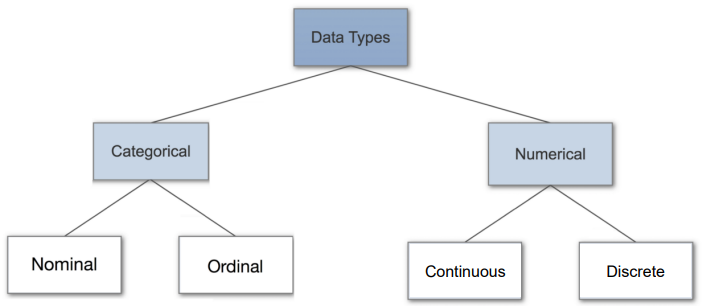
\includegraphics[width=\linewidth]{data_types.png}
\end{theorem}

\begin{corollary}{Nominal Data}
    \begin{itemize}
        \item Nominal scales are used for \textbf{labelling} variables, without any quantitative value
        \item No numerical significance
        \item Nominal data has no order
        \item Scales could simply be called labels
        \item Examples: gender, hair colour, race, marital status
    \end{itemize}
\end{corollary}

\begin{corollary}{Ordinal Data}
    \begin{itemize}
        \item Represents \textbf{discrete and ordered} units
        \item Nearly the same as nominal data, but \textbf{order matters}
        \item No distance between the different categories
        \item Examples: military rank, star rating, education level
    \end{itemize}
\end{corollary}

\begin{corollary}{Discrete Numeric Data}
    \begin{itemize}
        \item Represents items that can be \textbf{counted}
        \item Values may go from 0, 1, 2, on to infinity (making it countably infinite)
        \item Examples: number of persons in a room, number of "heads" in 60 coin flips, time elapsed in minutes
    \end{itemize}
\end{corollary}

\begin{corollary}{Continuous Numeric Data}
    \begin{itemize}
        \item Also known as \textbf{interval data}
        \item Often measurements
        \item Possible values \textbf{cannot be counted} and can only be described using intervals on the real number line
        \item Examples: temperature, weight, height, time, ...
    \end{itemize}
\end{corollary}

\begin{concept}{Overview Data Types}

    \textbf{Categorial Data}
    \begin{itemize}
        \item Nominal: no order, Scale ("labels") $\rightarrow$ e.g. hair colour, gender
        \item Ordinal: ordered $\rightarrow$ e.g. military rank, star rating
    \end{itemize}

    \textbf{Numerical Data} (ordered)
    \begin{itemize}
        \item Discrete: countable, ratio $\rightarrow$ e.g. number of persons in a room
        \item Continuous: interval, numeric scale $\rightarrow$ e.g. temperature, weight
    \end{itemize}
\end{concept}

\begin{definition}{Data Cleaning}
    is the process of improving the data quality by removing or improving incorrect or improperly formatted data.
    \vspace{2mm}\\
    \textbf{(near) duplicate detection} is the process of identifying and removing or merging duplicate data points.
    \begin{itemize}
        \item compare attributes of the tuple
        \item compare content of the attributes
    \end{itemize}

    \textbf{Filling missing values} is the process of replacing missing values with substituted values.
    \begin{itemize}
        \item ignore tuple
        \item fill in missing value manually
        \item use global constant such as "unknown" or "-1"
        \item use attribute mean, median, mode
        \item use most probable value
    \end{itemize}

    \textbf{Noisy data} is data with errors or outliers.
    \begin{itemize}
        \item Binning: divide the range of attribute values into bins
        \item Regression: smooth data by fitting the data into a function
        \item Clustering: detect and remove outliers
    \end{itemize}
\end{definition}

\begin{formula}{Binning}
    
    \textcolor{purple}{Equal Width Binning:}
    \begin{itemize}
        \item Divide the range into $N$ intervals of equal size (= width)
        \item $width = \frac{max - min}{N}$, $bin_i = [min + i \cdot width, min + (i+1) \cdot width]$
    \end{itemize}
    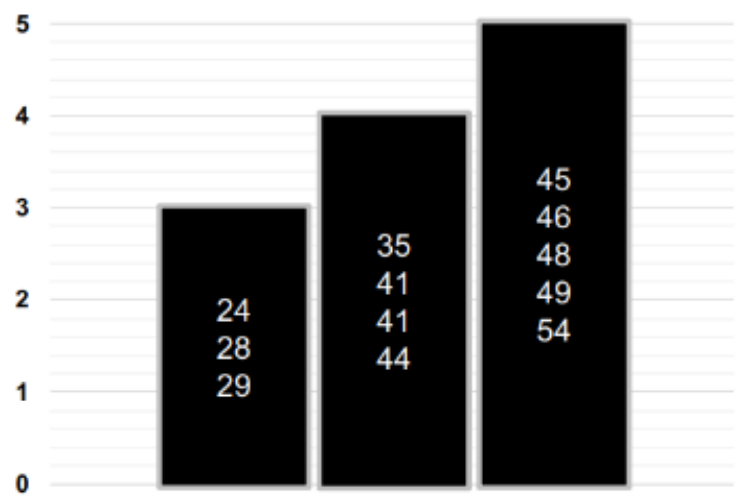
\includegraphics[width=0.5\linewidth]{equal_width_ninning.png}

    \textcolor{purple}{Equal Depth/Frequency Binning:}
    \begin{itemize}
        \item Divide the range into $N$ intervals with equal number of data points/records (= depth/frequency)
        \item $depth = \frac{N}{n}$, $bin_i = [data_{(i-1) \cdot depth}, data_{i \cdot depth}]$
    \end{itemize}
    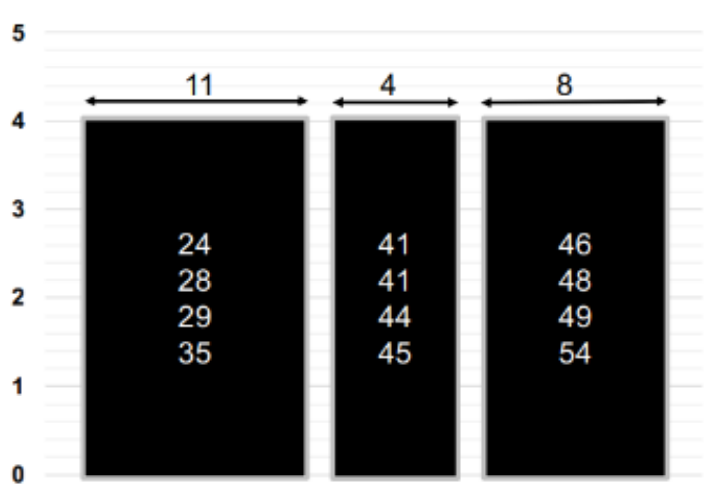
\includegraphics[width=0.5\linewidth]{equal_depth_binning.png}
\end{formula}

\begin{definition}{Linear Regression}
    Discover the parameters of the straight-line equation that best fits the data points.
    \begin{itemize}
        \item $\bar{x}$ is the mean value of $x$
        \item $\bar{y}$ is the mean value of $y$
    \end{itemize}
    $$
    b=\frac{\sum_{i=1}^n\left(x_i-\bar{x}\right)\left(y_i-\bar{y}\right)}{\sum_{i=1}^n\left(x_i-\bar{x}\right)^2}, \quad a=\bar{y}-b \bar{x}, \quad y=a+b x
    $$
    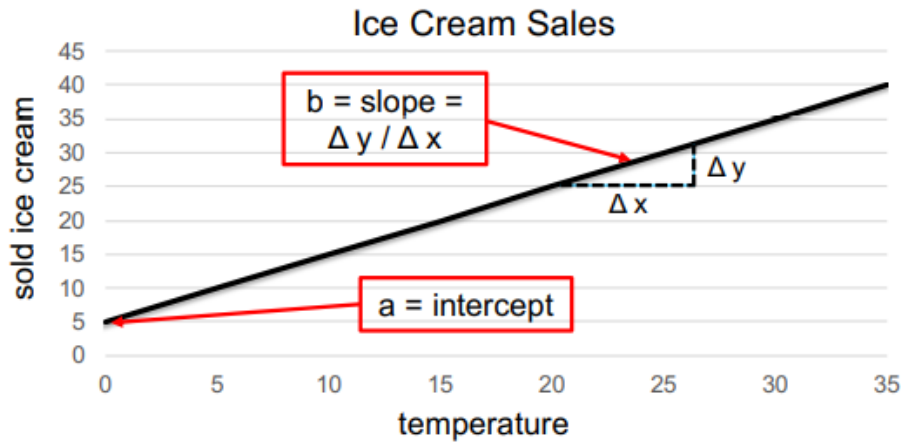
\includegraphics[width=\linewidth]{linear_regression_icecream.png}

    Usage: smooth out noise, fill in missing values, predict future/unknown values
\end{definition}

\begin{definition}{Data Normalization}
    is the process of transforming values of several variables into a similar range.
    \begin{itemize}
        \item Min-Max Normalization: $x_{norm} = \frac{x - min(x)}{max(x) - min(x)}$
        \item Z-Score Normalization: $x_{norm} = \frac{x - \bar{x}}{\sigma}$
    \end{itemize}
    
    Change the values of numeric columns to a common scale (e.g., between 0 and 1 ), without distorting differences in the ranges of values.
    \begin{itemize}
        \item Linear normalization: $f_{lin}(v) = \frac{v - min}{max - min}$
        \item Square root normalization: $f_{sq}(v) = \frac{\sqrt{v} - \sqrt{min}}{\sqrt{max} - \sqrt{min}}$
        \item Logarithmic normalization: $f_{ln}(v) = \frac{\ln(v) - \ln(min)}{\ln(max) - \ln(min)}$
    \end{itemize}

    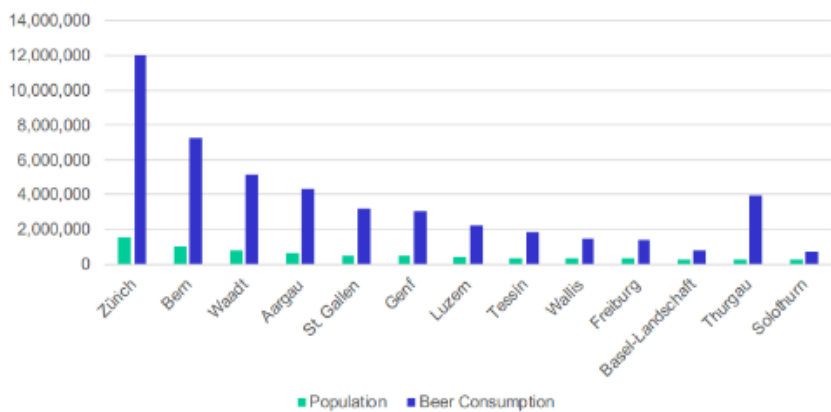
\includegraphics[width=0.5\linewidth]{data_normalization1.png}

    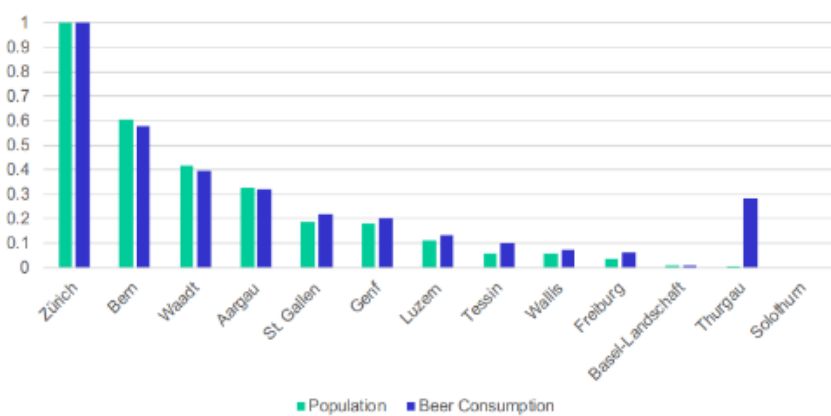
\includegraphics[width=0.5\linewidth]{data_normalization2.png}
\end{definition}

\begin{definition}{Data Sampling}
    Represent large dataset by smaller subset to speed up automatic calculations.
\textbf{Non-Probabilistic}
\begin{itemize}
    \item Convenience: easiest to obtain
    \item Judgement: based on experts' knowledge and judgement
    \item Snowball: purely based on referrals
    \item Quota: based on attribute values
\end{itemize}

\textbf{Probabilistic}
\begin{itemize}
    \item Simple Random: each item has an equal probability of being chosen
    \item Systematic: select some starting point and then select every $k$th element
    \item Stratified: divide the population into subgroups (strata) based on attributes and then draw a sample from each stratum
    \item Cluster: divide the population into clusters and then randomly select some of the clusters
\end{itemize}
\end{definition}

\begin{definition}{Data Partitioning}
    is the process of dividing the dataset into two or more parts.
    \begin{itemize}
        \item Training set: used to train the model
        \item Validation set: used to tune the model
        \item Test set: used to evaluate the model
    \end{itemize}

    \textcolor{pink}{\textbf{K-Fold Cross-Validation}}
    \begin{itemize}
        \item Divide the dataset into $k$ subsets (folds)
        \item Train the model $k$ times, each time using a different subset as the test set and the remaining points as the training set
        $\rightarrow$ train on k-1 folds, test on the remaining fold, repeat for each fold
        \item Average the results to get the final model $\rightarrow$ calculate average errors
    \end{itemize}
\end{definition}

\subsection{Evaluation}

\begin{formula}{Standard error measure}
    $$
    \begin{gathered}
    E=\frac{1}{N} \sum_{i=1}^N\left(1-\text { id }\left(\hat{y}_i, y_i\right)\right), \quad \text { id }(a, b)= \begin{cases}1 & \text { if } a=b \\
    0 & \text { else }\end{cases} \\
    \text { data } a_{\text {size }}=9, \quad \text { corret }=6, \quad \text { wrong }=3 \\
    E=\frac{1}{9} \cdot 3=0.33
    \end{gathered}
    $$
\end{formula}